%===========================================================================
%  Template for SunCar Focus Project, based on IDSC Master Thesis Template
%---------------------------------------------------------------------------
%
% Version 1
%
% 2010
%
%===========================================================================

% to compile this file for the first time, run
% latex, bibtex, latex, latex, dvips, ps2pdf

\documentclass[11pt,a4paper]{report}

% load the ethidsc package
\usepackage[english]{ethidsc}         % New styles and commands 
                                     % Options: - german or english

% load some more packages
\usepackage[latin1]{inputenc}        % encoding of tex files
\usepackage[english]{babel}          % hyphenation
\usepackage{amsmath}                 % Additional math functionality
%\usepackage{amssymb}                 % Additional math functionality
\usepackage{amsthm}                  % Additional math functionality
\usepackage{graphicx}                % EPS figures
\usepackage{fancyhdr}                % Headings
\usepackage{pstricks,pst-plot,psfrag}% Post-script graphics
\usepackage{multirow}                % Add functionality to tab. env.
\usepackage{rotating}                % Rotate tables 90 degrees
\usepackage{listings}                % Syntax specific code listing
\usepackage{mcode}                   % to include matlab code
%\usepackage{units}                   % Concise printing of units
\usepackage{SIunits}
\usepackage{longtable}         % Für Tabellen über mehrere Seiten
\usepackage{pdfpages}           % um PDF Seiten einzubinden
%\usepackage[authorformat=year,authorformat=italic,authorformat=and,titleformat=colonsep,titleformat=italic,commabeforerest]{jurabib} % for citations
\usepackage{caption}
\captionsetup{font={footnotesize}}
%\renewcommand*{\jbcitationyearformat}[1]{#1}
\usepackage[
bookmarks=true,         % show bookmarks bar
unicode=false,          % non-Latin characters in Acrobat's bookmarks
pdftoolbar=true,        % show Acrobat's toolbar?
pdfmenubar=true,        % show Acrobat's menu?
pdffitwindow=false,     % window fit to page when opened
pdfstartview={FitH},    % fits the width of the page to the window
pdftitle={Energetische Optimierung eines Photovoltaikmoduls durch aktive Kuehlung},
pdfauthor={Artemi Egorov},% title and author will be properties of the pdf
pdfnewwindow=true,      % links in new window
colorlinks=true,        % false: boxed links; true: colored links
linkcolor=black,        % color of internal links
citecolor=black,        % color of links to bibliography
filecolor=black,        % color of file links
urlcolor=black,         % color of external links
breaklinks=true         % break links across lines
]{hyperref}                          % Enable hyberrefs in PDF
\usepackage{breakurl}                % fixes a problem of hyperref and
                                     % makes urls break across lines

%\usepackage[]{natbib}

\usepackage{booktabs}
 
\usepackage{chngpage}

\usepackage[marginal,ragged]{footmisc} % fussnote: linksbündig, flattersatz

\fancypagestyle{plain}

% note: you can have more colorful links if you like
%\hypersetup{
%colorlinks=true,        % false: boxed links; true: colored links
%linkcolor=red,          % color of internal links
%citecolor=green,        % color of links to bibliography
%filecolor=magenta,      % color of file links
%urlcolor=cyan,          % color of external links
%}



%---------------------------------------------------------------------------

%\setlength{\parindent}{0em}                   % Disable parindent
\rhead[\nouppercase{\rightmark}]{\thepage}    % Special headings
\lhead[\thepage]{\nouppercase{\leftmark}}     % Special headings
\cfoot{}                                      % Special headings

%---------------------------------------------------------------------------

% customize the document with ethidsc commands

%\input{frontpage} % include definitions for front page

\declaration

%===========================================================================
\begin{document}

% list non-cited references
\nocite{ca_and_soc}
\nocite{sandpile_models}
\nocite{how_soc_works}
%\nocite{abelian_sandpile_model}


%---------------------------------------------------------------------------
% Title page

%\maketitle

% include title page pdf
%\includepdf[pages=1]{pdfs/titelblatt.pdf}

\thispagestyle{empty}

\begin{center}

\includegraphics[width=5cm]{ETHlogo.png}

\bigskip


\bigskip


\bigskip


\LARGE{ 	Lecture with Computer Exercises:\\ }
\LARGE{ Modelling and Simulating Social Systems with MATLAB\\}

\bigskip

\bigskip

\small{Project Report}\\

\bigskip

%\bigskip

%\bigskip

%\bigskip


\begin{tabular}{|c|}
\hline
\\
\textbf{\LARGE{Self-Organized Criticality in Sandpile Models}}\\
\\
\hline
\end{tabular}
\bigskip

\bigskip

\bigskip

% put a picture
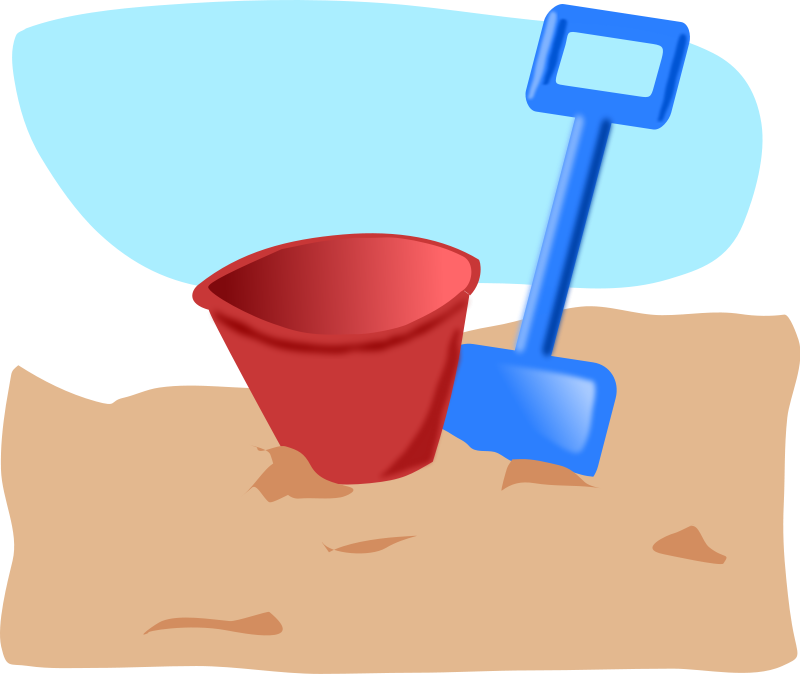
\includegraphics[width=8cm]{addon_bucket_and_spade.png}


\bigskip

\bigskip

\bigskip


\LARGE{Xinyi Chen \\ Artemi Egorov }





\bigskip

\bigskip

%\bigskip

%\bigskip

%\bigskip

Zurich\\
April 2012\\

\end{center}




\setboolean{@twoside}{true}  % change to two-side layout from here

\startnewchapter

% blank page
%\newpage
%\thispagestyle{empty}
%\mbox{}

\pagestyle{fancy}
\pagenumbering{roman}

% lesespalte 11.5 anstatt 12.5 [cm]
\changepage{0cm}{-1cm}{0.5cm}{0.5cm}{0cm}{0cm}{0cm}{0cm}{0cm}

%---------------------------------------------------------------------------
% Preamble

%!TEX root = bericht.tex
%!TEX encoding = latin1

%---------------------------------------------------------------------------
% Abstract



\phantomsection
\addcontentsline{toc}{chapter}{Abstract}
\chapter*{Abstract}

This paper describes the principles of self-organized criticallity and their validity in cellular automation models, in particular the sandpile model. The model, its diversity, its implementation in MATLAB/Octave with different parameters and its analysis are presented in detail. RESULTS ASDF?!?


\startnewchapter

% blank page
%\newpage
%\thispagestyle{empty}
%\mbox{}

%---------------------------------------------------------------------------
% Dankssagung

\phantomsection
\addcontentsline{toc}{chapter}{Acknowledgements}
\chapter*{Acknowledgements}

The project group would like to thank the \emph{Chair of Sociology, in particular of Modeling and Simulation}, for the chance to work on an interesting project and the possibility to apply simulation skills on extraordinary topics. Special thanks go to the assistants, namely Karsten Donnay and Stefano Balietti, for their all-time support during the project. Furthermore, the group would like to thank Pegah Kassraian Fard, who unfortunately had to quit the project, for her support in the early state of the project. Additional thanks go to the other groups of the class and of previous semesters.

\startnewchapter

%---------------------------------------------------------------------------
% Symbols

%\phantomsection
%\addcontentsline{toc}{chapter}{Nomenklatur}
%\chapter*{Nomenklatur}
%\label{chp:nomenklatur}

%\section*{Abk�rzungen}
%\begin{tabbing}
%\hspace*{1.6cm}\=\kill

%STC\> standard testing conditions\\[0.5ex]
%NX\> CAD, CAE und CAM Softwarepaket von Siemens

%\end{tabbing}


\startnewchapter

%---------------------------------------------------------------------------
% Table of contents

\setcounter{tocdepth}{2}
% create a bookmark that will appear in the booksmarks displayed by
% Adobe Reader, but not in the Table of Contents of the document
\label{TOC}
\pdfbookmark[0]{Table of contents}{TOC}
\tableofcontents


\startnewchapter

%---------------------------------------------------------------------------


\pagenumbering{arabic}
\newpage

%---------------------------------------------------------------------------
% Chapters

\chapter{to do list}
\thispagestyle{fancy}


\section{Individual contributions}

\section{Introduction and Motivations}

\section{Description of the Model}

\section{Implementation}

\section{Simulation Results and Discussion}

\section{Summary and Outlook}


%\include{}
%\startnewchapter




%---------------------------------------------------------------------------
% Literature
% (create .bib files using, for example, the free application Jabref)
% Compile your report in the following order: latex - bibtex - latex - latex
%\startnewchapter
\bibliographystyle{plain} % jurabib
\phantomsection
\addcontentsline{toc}{chapter}{References}
\begin{flushleft}
\bibliography{bibliography}
\end{flushleft}
\thispagestyle{fancy}

%---------------------------------------------------------------------------
% Appendix
\startnewchapter
\appendix
%!TEX root = bericht.tex
%!TEX encoding = latin1




%---------------------------------------------------------------------------

\startnewchapter

\chapter{MATLAB/Octave-Code}\label{chp:matlab}
\thispagestyle{fancy}
% NOTE: to change font size refer to mcode.sty

\section{``critical field.m'' - random field generation}
\lstinputlisting[frame=tb]{../../code/critical_field.m}
\vspace{2em}

\section{``sandpile.m'' - 2D sandpile model simulation, parametrized}
\lstinputlisting[frame=tb]{../../code/sandpile.m}
\vspace{2em}

\section{``avalanche distribution analysis.m''}
\lstinputlisting[frame=tb]{../../code/avalanche_distribution_analysis.m}
\vspace{2em}

\section{``test sandpile.m'' - sandpile simulation test environment}
\lstinputlisting[frame=tb]{../../code/test_sandpile.m}
\vspace{2em}

\section{``abelian sandpile.m'' - n-dimensional sandpile simulation w. friction}
\lstinputlisting[frame=tb]{../../code/xinyi/abelian_sandpile_XY.m}
\vspace{2em}

\section{``coordinate.m''}
\lstinputlisting[frame=tb]{../../code/xinyi/coordinate.m}
\vspace{2em}

\section{``linear index.m''}
\lstinputlisting[frame=tb]{../../code/xinyi/linear_index.m}
\vspace{2em}

\section{``neighbour.m''}
\lstinputlisting[frame=tb]{../../code/xinyi/neighbour.m}
\clearpage

%\section{Photothermie.m\cite{tyfocor}}
%\lstinputlisting[frame=tb]{matlab/photothermie1.m}
%\clearpage

%\section{Diffgleichung.m}
%\lstinputlisting[frame=tb]{matlab/photothermie2.m}
%\vspace{2em}



%---------------------------------------------------------------------------

\startnewchapter

%\chapter{Daten Oerlikon Solar PV-Modul}\label{appendix:oerlikon}
%\thispagestyle{fancy}

%\begin{itemize}
%\item Dimensionen: $1.1 \times 1.3$~m
%\item Wirkungsgrad: 8~\% (bei STC)
%\item Temperaturkoeffizient: -0.29~\%/K
%\end{itemize}

%\includepdf[pages=-]{pdfs/globalsolar_G2_Thin_Film_String_Datasheet.pdf}

 


\end{document}
%===========================================================================
